%% LyX 2.3.6.2 created this file.  For more info, see http://www.lyx.org/.
%% Do not edit unless you really know what you are doing.
\documentclass[english,aspectratio=169,handout]{beamer}
\usepackage{mathptmx}
\usepackage{eulervm}
\usepackage[T1]{fontenc}
\usepackage[latin9]{inputenc}
\usepackage{babel}
\usepackage{amstext}
\usepackage{amssymb}
\usepackage{graphicx}
\ifx\hypersetup\undefined
  \AtBeginDocument{%
    \hypersetup{unicode=true,pdfusetitle,
 bookmarks=true,bookmarksnumbered=false,bookmarksopen=false,
 breaklinks=false,pdfborder={0 0 0},pdfborderstyle={},backref=false,colorlinks=true,
 allcolors=NYUPurple,urlcolor=LightPurple}
  }
\else
  \hypersetup{unicode=true,pdfusetitle,
 bookmarks=true,bookmarksnumbered=false,bookmarksopen=false,
 breaklinks=false,pdfborder={0 0 0},pdfborderstyle={},backref=false,colorlinks=true,
 allcolors=NYUPurple,urlcolor=LightPurple}
\fi

\makeatletter

%%%%%%%%%%%%%%%%%%%%%%%%%%%%%% LyX specific LaTeX commands.
%% Because html converters don't know tabularnewline
\providecommand{\tabularnewline}{\\}

%%%%%%%%%%%%%%%%%%%%%%%%%%%%%% Textclass specific LaTeX commands.
% this default might be overridden by plain title style
\newcommand\makebeamertitle{\frame{\maketitle}}%
% (ERT) argument for the TOC
\AtBeginDocument{%
  \let\origtableofcontents=\tableofcontents
  \def\tableofcontents{\@ifnextchar[{\origtableofcontents}{\gobbletableofcontents}}
  \def\gobbletableofcontents#1{\origtableofcontents}
}

%%%%%%%%%%%%%%%%%%%%%%%%%%%%%% User specified LaTeX commands.
\usetheme{CambridgeUS} 
\beamertemplatenavigationsymbolsempty


% Set Color ==============================
\definecolor{NYUPurple}{RGB}{87,6,140}
\definecolor{LightPurple}{RGB}{165,11,255}


\setbeamercolor{title}{fg=NYUPurple}
%\setbeamercolor{frametitle}{fg=NYUPurple}
\setbeamercolor{frametitle}{fg=NYUPurple}

\setbeamercolor{background canvas}{fg=NYUPurple, bg=white}
\setbeamercolor{background}{fg=black, bg=NYUPurple}

\setbeamercolor{palette primary}{fg=black, bg=gray!30!white}
\setbeamercolor{palette secondary}{fg=black, bg=gray!20!white}
\setbeamercolor{palette tertiary}{fg=gray!20!white, bg=NYUPurple}

\setbeamertemplate{headline}{}

\setbeamercolor{parttitle}{fg=NYUPurple}
\setbeamercolor{sectiontitle}{fg=NYUPurple}
\setbeamercolor{sectionname}{fg=NYUPurple}
\setbeamercolor{section page}{fg=NYUPurple}

\AtBeginSection[]{
  \begin{frame}
    \frametitle{Table of Contents}
    \tableofcontents[currentsection]
  \end{frame}

  % \begin{frame}
  % \vfill
  % \centering
  % \begin{beamercolorbox}[sep=8pt,center,shadow=true,rounded=true]{title}
  %   \usebeamerfont{title}\insertsectionhead\par%
  % \end{beamercolorbox}
  % \vfill
  % \end{frame}
}

\makeatother

\begin{document}
\global\long\def\reals{\mathbf{R}}%
 
\global\long\def\integers{\mathbf{Z}}%
 
\global\long\def\naturals{\mathbf{N}}%
 
\global\long\def\rationals{\mathbf{Q}}%
 
\global\long\def\ca{\mathcal{A}}%
 
\global\long\def\cb{\mathcal{B}}%
 
\global\long\def\cc{\mathcal{C}}%
 
\global\long\def\cd{\mathcal{D}}%
 
\global\long\def\ce{\mathcal{E}}%
 
\global\long\def\cf{\mathcal{F}}%
 
\global\long\def\cg{\mathcal{G}}%
 
\global\long\def\ch{\mathcal{H}}%
 
\global\long\def\ci{\mathcal{I}}%
 
\global\long\def\cj{\mathcal{J}}%
 
\global\long\def\ck{\mathcal{K}}%
 
\global\long\def\cl{\mathcal{L}}%
 
\global\long\def\cm{\mathcal{M}}%
 
\global\long\def\cn{\mathcal{N}}%
 
\global\long\def\co{\mathcal{O}}%
 
\global\long\def\cp{\mathcal{P}}%
 
\global\long\def\cq{\mathcal{Q}}%
 
\global\long\def\calr{\mathcal{R}}%
 
\global\long\def\cs{\mathcal{S}}%
 
\global\long\def\ct{\mathcal{T}}%
 
\global\long\def\cu{\mathcal{U}}%
 
\global\long\def\cv{\mathcal{V}}%
 
\global\long\def\cw{\mathcal{W}}%
 
\global\long\def\cx{\mathcal{X}}%
 
\global\long\def\cy{\mathcal{Y}}%
 
\global\long\def\cz{\mathcal{Z}}%
 
\global\long\def\ind#1{1(#1)}%
 %\newcommand{\pr}{P}
\global\long\def\pr{\mathbb{P}}%
 
\global\long\def\predsp{\cy}%
 %{\hat{\cy}}
\global\long\def\outsp{\cy}%

\global\long\def\prxy{P_{\cx\times\cy}}%
 
\global\long\def\prx{P_{\cx}}%
 
\global\long\def\prygivenx{P_{\cy\mid\cx}}%
 %\newcommand{\ex}{E}
\global\long\def\ex{\mathbb{E}}%
 
\global\long\def\var{\textrm{Var}}%
 
\global\long\def\cov{\textrm{Cov}}%
 
\global\long\def\sgn{\textrm{sgn}}%
 
\global\long\def\sign{\textrm{sign}}%
 
\global\long\def\kl{\textrm{KL}}%
 
\global\long\def\law{\mathcal{L}}%
 
\global\long\def\eps{\varepsilon}%
 
\global\long\def\as{\textrm{ a.s.}}%
 
\global\long\def\io{\textrm{ i.o.}}%
 
\global\long\def\ev{\textrm{ ev.}}%
 
\global\long\def\convd{\stackrel{d}{\to}}%
 
\global\long\def\eqd{\stackrel{d}{=}}%
 
\global\long\def\del{\nabla}%
 
\global\long\def\loss{\ell}%
 
\global\long\def\risk{R}%
 
\global\long\def\emprisk{\hat{R}}%
 
\global\long\def\lossfnl{L}%
 
\global\long\def\emplossfnl{\hat{L}}%
 
\global\long\def\empminimizer#1{\hat{#1}^{*}}%
 
\global\long\def\minimizer#1{#1^{*}}%
\global\long\def\optimizer#1{#1^{*}}%
 
\global\long\def\etal{\textrm{et. al.}}%
 
\global\long\def\tr{\operatorname{tr}}%

\global\long\def\trace{\operatorname{trace}}%
 
\global\long\def\diag{\text{diag}}%
 
\global\long\def\rank{\text{rank}}%
 
\global\long\def\linspan{\text{span}}%
 
\global\long\def\spn{\text{span}}%
 
\global\long\def\proj{\text{Proj}}%
 
\global\long\def\argmax{\operatornamewithlimits{arg\, max}}%
 
\global\long\def\argmin{\operatornamewithlimits{arg\, min}}%

\global\long\def\bfx{\mathbf{x}}%
 
\global\long\def\bfy{\mathbf{y}}%
 
\global\long\def\bfl{\mathbf{\lambda}}%
 
\global\long\def\bfm{\mathbf{\mu}}%
 
\global\long\def\calL{\mathcal{L}}%

\global\long\def\vw{\boldsymbol{w}}%
 
\global\long\def\vx{\boldsymbol{x}}%
 
\global\long\def\vxi{\boldsymbol{\xi}}%
 
\global\long\def\valpha{\boldsymbol{\alpha}}%
 
\global\long\def\vbeta{\boldsymbol{\beta}}%
 
\global\long\def\vsigma{\boldsymbol{\sigma}}%
\global\long\def\vtheta{\boldsymbol{\theta}}%
 
\global\long\def\vd{\boldsymbol{d}}%
 
\global\long\def\vs{\boldsymbol{s}}%
 
\global\long\def\vt{\boldsymbol{t}}%
 
\global\long\def\vh{\boldsymbol{h}}%
 
\global\long\def\ve{\boldsymbol{e}}%
 
\global\long\def\vf{\boldsymbol{f}}%
 
\global\long\def\vg{\boldsymbol{g}}%
 
\global\long\def\vz{\boldsymbol{z}}%
 
\global\long\def\vk{\boldsymbol{k}}%
 
\global\long\def\va{\boldsymbol{a}}%
 
\global\long\def\vb{\boldsymbol{b}}%
 
\global\long\def\vv{\boldsymbol{v}}%
 
\global\long\def\vy{\boldsymbol{y}}%

\global\long\def\dom{\textrm{\textbf{dom} }}%
\global\long\def\rank{\text{\textbf{rank }}}%
\global\long\def\conv{\textrm{\textbf{conv} }}%
\global\long\def\relint{\text{\textbf{relint }}}%
\global\long\def\aff{\text{\textbf{aff }}}%

\global\long\def\hil{\ch}%
 
\global\long\def\rkhs{\hil}%
 
\global\long\def\ber{\text{Ber}}%

\global\long\def\softmax{\text{Softmax}}%

\title[DS-GA 1003 ]{Probabilistic models\\
- \\
Conditional Probability Models}
\author{Marylou Gabri\'e \\
Slides based on Lecture
\href{https://github.com/davidrosenberg/mlcourse/blob/gh-pages/Lectures/06c.conditional-probability-models.pdf}{06c} from David Rosenberg's course materials (\url{https://github.com/davidrosenberg/mlcourse})}
\date{March 9, 2021}
\institute{CDS, NYU}

\makebeamertitle
\mode<article>{Just in article version}

\begin{frame}{Contents}

\tableofcontents{}
\end{frame}

\section{Modeling Conditional Distributions - Linear Predictors}
\begin{frame}{Conditional Distribution Estimation (Generalized Regression)}

\begin{itemize}
\item Task: Given $x$, predict probability distribution $p(y| x)$

\pause{}
\item Method:
\begin{enumerate}
  \item Represent $p(y| x)$ with \emph{parametric families} of distributions: $p(y ; \theta(x))$ with parameters $\theta$.
  \item Maximize likelihood of training data: $\hat{\theta}  \in \argmax_{\theta}\log p(\cd,\hat{\theta})$
\end{enumerate} 

\pause{}
\item Examples:
\begin{enumerate}
\item Logistic regression (Bernoulli distribution)

\pause{}
\item Poisson regression (Poisson distribution)

\pause{}
\item Linear regression (Normal distribution, fixed variance)

\pause{}
\item Gradient Boosting Machines (GBM) {[}in a few weeks{]}

\pause{}
\item Many neural network models used in practice (though this is
not their essential feature)
\end{enumerate}
\end{itemize}
\end{frame}
%

\begin{frame}{Linear Probabilistic Classifiers}
  \begin{itemize}
  \item Setting: $\cx=\reals^{d}$, $\cy$ arbitrary for now
  \item Want prediction function to map each $x\in\reals^{d}$ to $\theta\in\Theta$ for $p(y ; \theta(x))$.
  
  \pause{}
 
  \item For a \textbf{linear method}, we first \textbf{extract} \textbf{information }from $x\in\reals^{d}$
  and summarize in a single number with a linear
  function:
  \[
  \underbrace{x}_{\in\reals^{d}}\mapsto\underbrace{w^{T}x}_{\in\reals}
  \]
  (That number is analogous to the \textbf{score} in classification.
  )
  \pause{}
  \item As usual, $x\mapsto w^{T}x$ will include affine functions if we include
  a constant feature in $x$.
  
  \pause{}
  \item $w^{T}x$ is called the \textbf{linear predictor. }
  \item Still need to map this to $\Theta$.
  \end{itemize}
  \end{frame}
  %
  \begin{frame}{The Transfer Function}
  \begin{itemize}
  \item Need a function to map the linear predictor in $\reals$ to $\Theta$:
  \[
  \underbrace{x}_{\in\reals^{d}}\mapsto\underbrace{w^{T}x}_{\in\reals}\mapsto\pause\underbrace{f(w^{T}x)}_{\in\Theta}=\theta,
  \]
  where $f:\reals\to\Theta$. We'll call $f$ the \textbf{transfer }function.
  \end{itemize}
  
  \pause{}
  \begin{itemize}
  \item So prediction function is $x\mapsto f(w^{T}x)$.
  \item The prediction function gives us the parameter for $p(y ; \theta(x))$ used to estimate $p(y|x)$.
  \pause{}
  \item Later in the course we will use some non linear predictors, but not today.
  \end{itemize}
  
  \end{frame}
  %

  \begin{frame}{Contents}

    \tableofcontents{}
  \end{frame}


\section{Bernoulli Regression}
\begin{frame}{Probabilistic Binary Classifiers}
\begin{itemize}
\item Setting: $\cx=\reals^{d}$, $\cy=\left\{ 0,1\right\} $

\pause{}
\item For each $x$, need to predict a distribution on $\cy=\left\{ 0,1\right\} $.
\item How can we define a distribution supported on $\left\{ 0,1\right\} $?

\pause{}
\item Sufficient to specify the \textbf{Bernoulli parameter} $\theta=p(y=1)$.

\pause{}
\item We can refer to this distribution as $\text{Bernoulli}(\theta)$.
\end{itemize}
\end{frame}
%

\begin{frame}{Transfer Functions for Bernoulli}

\begin{itemize}
\item Two commonly used transfer functions to map from $w^{T}x$ to $\theta$:
\end{itemize}
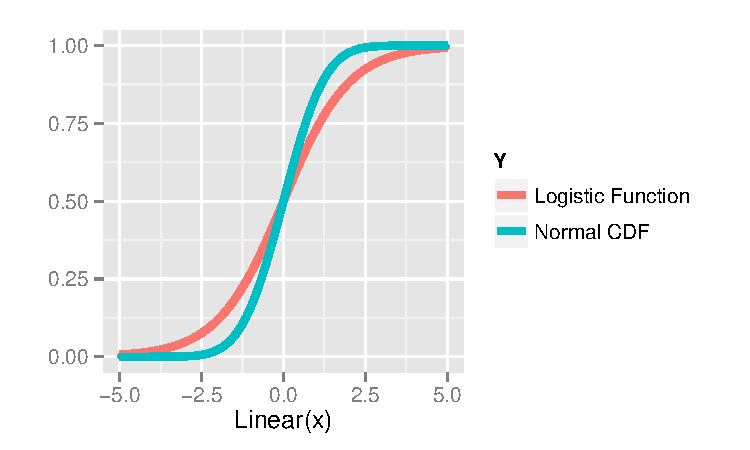
\includegraphics[width=0.6\textwidth]{figs/bernoulliInverseLinkFunctions}
\begin{itemize}
\item Logistic function: $f(\eta)=\frac{1}{1+e^{-\eta}}$ $\pause\implies$
Logistic Regression
\item Normal CDF $f(\eta)=\int_{-\infty}^{\eta}\frac{1}{\sqrt{2\pi}}e^{-x^{2}/2}$$\pause\implies$
Probit Regression
\end{itemize}
\end{frame}
%
\begin{frame}{Learning}

\begin{itemize}
\item Input space $\cx=\reals^{d}$
\item Outcome space $\cy=\left\{ 0,1\right\} $

% \pause{}
\item Action space $\ca=\Theta=[0,1]$ (Representing Bernoulli$(\theta)$ distributions
by $\theta\in\left[0,1\right]$)

\pause{}
\item Hypothesis space $\cf=\left\{ x\mapsto f(w^{T}x)\mid w\in\reals^{d}\right\} $ 

\pause{}
\item Parameter space $\reals^{d}$ (Each prediction function represented
by $w\in\reals^{d}.)$

\pause{}
\item We can choose $w$ using maximum likelihood...
\end{itemize}
\end{frame}
%
\begin{frame}{Bernoulli Regression: Likelihood Scoring Example}
\begin{itemize}
\item Suppose we have $\cx=\reals$ and data $\cd$: $(-3,0),\left(0,0\right),(1,1),(2,0)\in\reals\times\left\{ 0,1\right\} $

\pause{}
\item Our model is $p(y=1\mid x)=f(wx)$, for some parameter $w\in\reals$.

\pause{}
\item Compute the likelihood for each observation:
\end{itemize}
\begin{center}
\begin{tabular}{|c|c|c|c|c|}
\hline 
$x$ & $y$ & $wx$ & $\theta=f(wx)$ & $\hat{p}(y)$\tabularnewline
\hline 
\hline 
$-3$ & $0$ & $-3w$ & $f(-3w)$ & $1-f(-3w)$\tabularnewline
\hline 
$0$ & $0$ & $0$ & $f(0)$ & $1-f(0)$\tabularnewline
\hline 
$1$ & $1$ & $w$ & $f(w)$ & $f(w)$\tabularnewline
\hline 
$2$ & $0$ & $2w$ & $f(2w)$ & $1-f(2w)$\tabularnewline
\hline 
\end{tabular}
\par\end{center}

\pause{}
\begin{itemize}
\item The likelihood of $w$ for the data $\cd$ is
\[
p(\cd;w)=\left[1-f(-3w)\right]\cdot\left[1-f(0)\right]\cdot\left[f(w)\right]\cdot\left[1-f(2w)\right]
\]
\end{itemize}

\pause{}
\begin{itemize}
\item The MLE $\hat{w}$ is the $w\in\reals$ maximizing $p(\cd;w)$ for
the given $\cd$. 
\end{itemize}
\end{frame}
%
\begin{frame}{A Clever Way To Write $\hat{p}(y\mid x;w)$}
\begin{itemize}
\item For a given $x,w\in\reals^{d}$ and $y\in\left\{ 0,1\right\} $, the
likelihood of $w$ for $\left(x,y\right)$ is
\[
p(y\mid x;w)=\pause\begin{cases}
f(w^{T}x) & y=1\\
1-f(w^{T}x) & y=0
\end{cases}
\]
\end{itemize}

\pause{}
\begin{itemize}
\item It will be convenient to write this as
\[
p(y\mid x;w)=\left[f(w^{T}x)\right]^{y}\left[1-f(w^{T}x)\right]^{1-y}\pause,
\]
which is obvious as long as you remember $y\in\left\{ 0,1\right\} $.
\end{itemize}
\end{frame}
%
\begin{frame}{Bernoulli Regression: Likelihood Scoring}
\begin{itemize}
\item Suppose we have data $\cd:\;(x_{1},y_{1}),\ldots,(x_{n},y_{n})\in\reals^{d}\times\left\{ 0,1\right\} $.

\pause{}
\item The likelihood of $w\in\reals^{d}$ for data $\cd$ is
\begin{eqnarray*}
p(\cd;w) & = & \prod_{i=1}^{n}p(y_{i}\mid x_{i};w)\text{ [by independence]}\\
\pause & = & \prod_{i=1}^{n}\left[f(w^{T}x_{i})\right]^{y_{i}}\left[1-f(w^{T}x_{i})\right]^{1-y_{i}}.
\end{eqnarray*}


\pause{}
\item Easier to work with the log-likelihood:
\[
\log p(\cd;w)=\sum_{i=1}^{n}\left(y_{i}\log f(w^{T}x_{i})+\left(1-y_{i}\right)\log\left[1-f(w^{T}x_{i})\right]\right)
\]
\end{itemize}
\end{frame}
%
\begin{frame}{Bernoulli Regression: MLE}
\begin{itemize}
\item Maximum Likelihood Estimation (MLE) finds $w$ maximizing $\log p(\cd;w)$.

\pause{}
\item Equivalently, minimize the \textbf{negative log-likelihood} objective
function
\[
J(w)=-\left[\sum_{i=1}^{n}y_{i}\log f(w^{T}x_{i})+\left(1-y_{i}\right)\log\left[1-f(w^{T}x_{i})\right]\right].
\]


\pause{}
\item For differentiable $f$,
\begin{itemize}
\item $J(w)$ is differentiable, and we can use our standard tools. 
\item In labs, already derived the SGD step directions for logistic regression.
\item Possible {[}harder{]} homework: derived the SGD step directions for probit regression.
\end{itemize}

\end{itemize}

\end{frame}

\section{Poisson Regression}

\global\long\def\poi{\text{Poisson}}%

\begin{frame}{Poisson Regression: Setup}
\begin{itemize}
\item Input space $\cx=\reals^{d}$, Output space $\cy=\left\{ 0,1,2,3,4,\dots\right\} $

\pause{}
\item In Poisson regression, prediction functions produce a Poisson distribution.
\begin{itemize}
\item Represent Poisson$\left(\lambda\right)$ distribution by the mean
parameter $\lambda\in\left(0,\infty\right)$.

\pause{}
\end{itemize}
\item Action space $\ca=\left(0,\infty\right)$

\pause{}
\item In Poisson regression, $x$ enters \textbf{linearly:} $x\mapsto\underbrace{w^{T}x}_{\reals}\mapsto\lambda=\underbrace{f(w^{T}x)}_{(0,\infty)}$.

\pause{}
\item What can we use as the transfer function $f:\reals\to\left(0,\infty\right)$?
\end{itemize}
\end{frame}
%
\begin{frame}{Poisson Regression: Transfer Function}
\begin{itemize}
\item In Poisson regression, $x$ enters \textbf{linearly:} 
\[
x\mapsto\underbrace{w^{T}x}_{\reals}\mapsto\lambda=\underbrace{f(w^{T}x)}_{(0,\infty)}.
\]
\item Standard approach is to take
\[
f(w^{T}x)=\exp\left(w^{T}x\right).
\]


\pause{}
\item Note that range of $f(w^{T}x)\in\left(0,\infty\right)$, (appropriate
for the Poisson parameter).
\end{itemize}
\end{frame}
%
\begin{frame}{Poisson Regression: Likelihood Scoring}
\begin{itemize}
\item Suppose we have data $\cd=\left\{ (x_{1},y_{1}),\ldots,(x_{n},y_{n})\right\} $.
\item Recall the log-likelihood for Poisson parameter $\lambda_{i}$ on
observation $y_{i}$ is:
\begin{eqnarray*}
\log p(y_{i};\lambda_{i}) & = & \left[y_{i}\log\lambda_{i}-\lambda_{i}-\log\left(y_{i}!\right)\right]
\end{eqnarray*}


\pause{}
\item Now we want to predict a different $\lambda_{i}$ for every $x_{i}$
with the model
\[
\lambda_{i}=f(w^{T}x_{i})=\exp\left(w^{T}x_{i}\right).
\]


\pause{}
\item The likelihood for $w$ on the full dataset $\cd$ is
\begin{eqnarray*}
\log p(\cd;w) & = & \sum_{i=1}^{n}\left[y_{i}\log\left[\exp\left(w^{T}x_{i}\right)\right]-\exp\left(w^{T}x_{i}\right)-\log\left(y_{i}!\right)\right]\\
 & = & \sum_{i=1}^{n}\left[y_{i}w^{T}x_{i}-\exp\left(w^{T}x_{i}\right)-\log\left(y_{i}!\right)\right]
\end{eqnarray*}
\end{itemize}
\end{frame}
%
\begin{frame}{Poisson Regression: MLE}
\begin{itemize}
\item To get MLE, need to maximize 
\[
J(w)=\log p(\cd;w)=\sum_{i=1}^{n}\left[y_{i}w^{T}x_{i}-\exp\left(w^{T}x_{i}\right)-\log\left(y_{i}!\right)\right]
\]
 over $w\in\reals^{d}$.
\end{itemize}

\pause{}
\begin{itemize}
\item No closed form for optimum, but it's concave, so easy to optimize. 
\end{itemize}
\end{frame}
%
\begin{frame}{Poisson Regression Example}

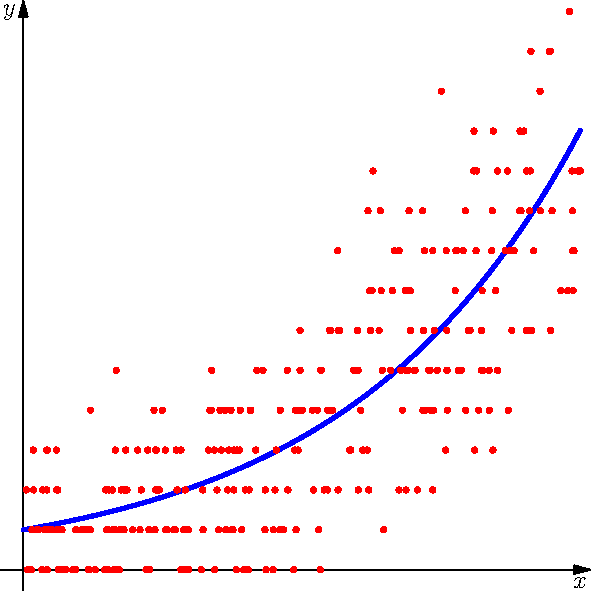
\includegraphics[height=0.55\paperheight]{figs/poissonBumps2}
\begin{itemize}
\item Example application: Phone call counts per day for a startup company,
over 300 days.

\pause{}
\item Blue line is mean $\mu(x)=\exp\left(wx\right)$, some $w\in\reals\pause$.
(Only linear part $x\mapsto wx$ is learned.)

\pause{}
\item Samples are $y_{i}\sim\text{Poisson}(wx_{i})$. \let\thefootnote\relax\footnotetext{\tiny{Plot courtesy of Brett Bernstein.}}
\end{itemize}
\end{frame}
%
\begin{frame}{Nonlinear Score Function: Sneak Preview}
 

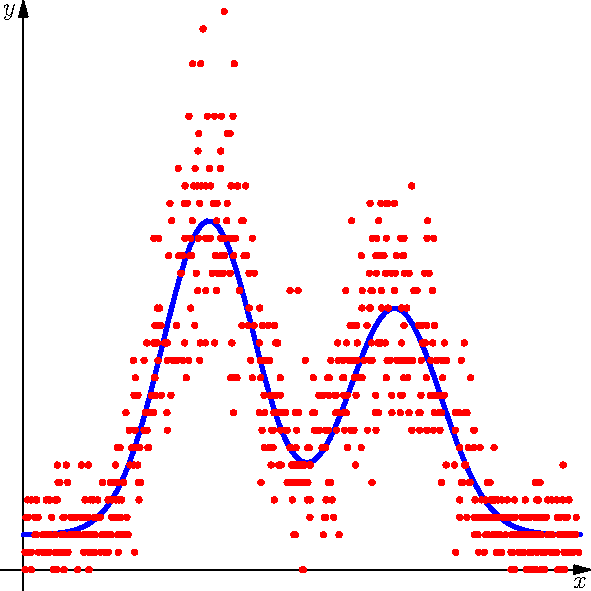
\includegraphics[height=0.55\paperheight]{figs/poissonBumps}
\begin{itemize}
\item Blue line is mean $\mu(x)=\exp\left(f(x)\right)$, for some nonlinear
$f$ learned from data.

\pause{}
\item Samples are $y_{i}\sim\text{Poisson}(\exp\left(f(x_{i})\right)$.

\pause{}
\item We can do this with gradient boosting and neural networks, coming
up in a few weeks. \let\thefootnote\relax\footnotetext{\tiny{Plot courtesy of Brett Bernstein.}}
\end{itemize}
\end{frame}
%

\section{Conditional Gaussian Regression}
\begin{frame}{Gaussian Linear Regression}
\begin{itemize}
\item Input space $\cx=\reals^{d}$, Output space $\cy=\reals$

\pause{}
\item In Gaussian regression, prediction functions produce a distribution
$\cn(\mu,\sigma^{2})$.
\begin{itemize}
\item Assume $\sigma^{2}$ is known.
\end{itemize}
\item Represent $\cn(\mu,\sigma^{2})$ by the mean parameter $\mu\in\reals$.

\pause{}
\item Action space $\ca=\reals$

\pause{}
\item In Gaussian linear regression, $x$ enters \textbf{linearly:} $x\mapsto\underbrace{w^{T}x}_{\reals}\mapsto\mu=\underbrace{f(w^{T}x)}_{\reals}$.

\pause{}
\item Since $\mu\in\reals$, we can take the identity transfer function:
$f(w^{T}x)=w^{T}x$.
\end{itemize}
\end{frame}
%
\begin{frame}{Gaussian Regression: Likelihood Scoring}
\begin{itemize}
\item Suppose we have data $\cd=\left\{ (x_{1},y_{1}),\ldots,(x_{n},y_{n})\right\} $.
\item Compute the model likelihood for $\cd$:
\begin{align*}
p(\cd;w)= & \prod_{i=1}^{n}p(y_{i}\mid x_{i};w)\text{ [by independence]}
\end{align*}


\pause{}
\item Maximum Likelihood Estimation (MLE) finds $w$ maximizing $\hat{p}(\cd;w)$.
\item Equivalently, maximize the data log-likelihood:
\[
\minimizer w=\argmax_{w\in\reals^{d}}\sum_{i=1}^{n}\log p(y_{i}\mid x_{i};w)
\]


\pause{}
\item Let's start solving this!
\end{itemize}
\end{frame}
%
\begin{frame}{Gaussian Regression: MLE}
\begin{itemize}
\item The conditional log-likelihood is:
\begin{eqnarray*}
 &  & \sum_{i=1}^{n}\log p(y_{i}\mid x_{i};w)\\
\pause & = & \sum_{i=1}^{n}\log\left[\frac{1}{\sigma\sqrt{2\pi}}\exp\left(-\frac{(y_{i}-w^{T}x_{i})^{2}}{2\sigma^{2}}\right)\right]\\
\pause & = & \underbrace{\sum_{i=1}^{n}\log\left[\frac{1}{\sigma\sqrt{2\pi}}\right]}_{\mbox{independent of }w}+\sum_{i=1}^{n}\left(-\frac{(y_{i}-w^{T}x_{i})^{2}}{2\sigma^{2}}\right)
\end{eqnarray*}


\pause{}
\begin{itemize}
\item MLE is the $w$ where this is maximized.

\pause{}
\item Note that $\sigma^{2}$ is irrelevant to finding the maximizing $w$.

\pause{}
\item Can drop the negative sign and make it a minimization problem.
\end{itemize}
\end{itemize}
\end{frame}
%
\begin{frame}{Gaussian Regression: MLE}
\begin{itemize}
\item The MLE is 
\begin{align*}
\minimizer w= & \argmin_{w\in\reals^{d}}\sum_{i=1}^{n}(y_{i}-w^{T}x_{i})^{2}
\end{align*}


\pause{}
\item This is exactly the objective function for least squares. 
\item We provided a probabilistic interpretation of the least square objective.

\pause{}
\item From here, can use usual approaches to solve for $w^{*}$ (SGD, linear
algebra, calculus, etc.) 
\end{itemize}

\end{frame}
%

\section{Multinomial Logistic Regression}
\begin{frame}{Multinomial Logistic Regression}
\begin{itemize}
\item Setting: $\cx=\reals^{d}$, $\cy=\left\{ 1,\ldots,k\right\} $
\end{itemize}

\pause{}
\begin{itemize}
\item For each $x$, we want to produce a distribution on $k$ classes.
\end{itemize}

\pause{}
\begin{itemize}
\item Such a distribution is called a ``\textbf{multinoulli}'' or ``\textbf{categorical}''
distribution.
\end{itemize}

\pause{}
\begin{itemize}
\item Represent categorical distribution by probability vector $\theta=\left(\theta_{1},\ldots,\theta_{k}\right)\in\reals^{k}$:
\begin{itemize}
\item $\sum_{i=1}^{k}\theta_{i}=1$ and $\theta_{i}\ge0$ for $i=1,\ldots,k$
\item i.e. $\theta$ represents a \textbf{discrete distribution}) 
\end{itemize}

\pause{}
\item So $\forall y\in\left\{ 1,\ldots,k\right\} $, $p(y)=\theta_{y}$.
\end{itemize}
\end{frame}
%
\begin{frame}{Multinomial Logistic Regression}
\begin{itemize}
\item From each $x$, we compute a linear score function for each class:
\[
x\mapsto\left(\left\langle w_{1},x\right\rangle ,\ldots,\left\langle w_{k},x\right\rangle \right)\in\reals^{k},
\]
where we've introduced parameter vectors $w_{1},\ldots,w_{k}\in\reals^{d}$.

\pause{}
\item We need to map this $\reals^{k}$ vector of scores into a probability
vector.

\pause{}
\item Consider the \textbf{softmax function:
\[
\left(s_{1},\ldots,s_{k}\right)\mapsto\theta=\left(\frac{e^{s_{1}}}{\sum_{i=1}^{k}e^{s_{i}}},\ldots,\frac{e^{s_{k}}}{\sum_{i=1}^{k}e^{s_{i}}}\right).
\]
}

\pause{}
\item Note that $\theta\in\reals^{k}$ and
\begin{eqnarray*}
\theta_{i} & > & 0\qquad i=1,\ldots,k\\
\sum_{i=1}^{k}\theta_{i} & = & 1
\end{eqnarray*}
\end{itemize}
\end{frame}
%
\begin{frame}{Multinomial Logistic Regression}
\begin{itemize}
\item Say we want to get the predicted categorical distribution for a given
$x\in\reals^{d}$. 
\item First compute the scores $(\in\reals^{k})$ and then their softmax:
\textbf{
\[
x\mapsto\left(\left\langle w_{1},x\right\rangle ,\ldots,\left\langle w_{k},x\right\rangle \right)\mapsto\theta=\left(\frac{\exp\left(w_{1}^{T}x\right)}{\sum_{i=1}^{k}\exp\left(w_{i}^{T}x\right)},\ldots,\frac{\exp\left(w_{k}^{T}x\right)}{\sum_{i=1}^{k}\exp\left(w_{i}^{T}x\right)}\right)
\]
}
\end{itemize}

\pause{}
\begin{itemize}
\item We can write the conditional probability for any $y\in\left\{ 1,\ldots,k\right\} $
as
\[
p(y\mid x;w)=\frac{\exp\left(w_{y}^{T}x\right)}{\sum_{i=1}^{k}\exp\left(w_{i}^{T}x\right)}.
\]
\end{itemize}
\end{frame}
%
\begin{frame}{Multinomial Logistic Regression}
\begin{itemize}
\item Putting this together, we write multinomial logistic regression as
\[
p(y\mid x;w)=\frac{\exp\left(w_{y}^{T}x\right)}{\sum_{i=1}^{k}\exp\left(w_{i}^{T}x\right)}.
\]


\pause{}
\item How do we do learning here? What parameters are we estimating?

\pause{}
\item Our model is specified once we have $w_{1},\ldots,w_{k}\in\reals^{d}$.
\item Find parameter settings maximizing the log-likelihood of data $\cd$.

\pause{}
\item This objective function is concave in $w$'s and straightforward to
optimize.
\end{itemize}
\end{frame}

\section{Maximum Likelihood as ERM}
\begin{frame}{Conditional Probability Modeling as Statistical Learning}

\begin{itemize}
\item Input space $\cx$
\item Outcome space $\cy$
\item All pairs $(x,y)$ are independent with distribution $P_{\cx\times\cy}$. 

\pause{}
\item \textbf{Action space} $\ca=\left\{ p(y)\mid p\text{ is a probability density or mass function on }\cy\right\} $.

\pause{}
\item Hypothesis space $\cf$ contains decision functions $f:\cx\to\ca$. 

\pause{}
\item Maximum likelihood estimation for dataset $\cd=\left((x_{1},y_{1}),\ldots,(x_{n},y_{n}\right)$
is
\[
\hat{f}_{\text{MLE}}\in\argmax_{f\in\cf}\sum_{i=1}^{n}\log\left[f(x_{i})(y_{i})\right]
\]


\pause{}
\begin{exampleblock}{Exercise}

Write the MLE optimization as empirical risk minimization. What's
the loss?
\end{exampleblock}
\end{itemize}
\end{frame}
%
\begin{frame}{Conditional Probability Modeling as Statistical Learning}

\begin{itemize}
\item Take loss $\ell:\ca\times\cy\to\reals$ for a predicted PDF or PMF
$p(y)$ and outcome $y$ to be
\[
\ell(p,y)=-\log p(y)
\]


\pause{}
\item The risk of decision function $f:\cx\to\ca$ is
\[
R(f)=-\ex_{x,y}\log\left[f(x)(y)\right],
\]
where $f(x)$ is a PDF or PMF on $\cy$, and we're evaluating it on
$y$.
\end{itemize}
\end{frame}
%
\begin{frame}{Conditional Probability Modeling as Statistical Learning}
\begin{itemize}
\item The empirical risk of $f$ for a sample $\cd=\left\{ y_{1},\ldots,y_{n}\right\} \in\cy$
is 
\[
\hat{R}(f)=-\frac{1}{n}\sum_{i=1}^{n}\log\left[f(x_{i})(y_{i})\right].
\]
This is called the negative \textbf{conditional log-likelihood}.
\end{itemize}

\pause{}
\begin{itemize}
\item Thus for the negative log-likelihood loss, ERM and MLE are equivalent
\end{itemize}
\end{frame}


\end{document}
